\documentclass[a4paper, 14pt]{extarticle}

%% Pacotes Gerais %%
\usepackage[utf8]{inputenc}
\usepackage[T1]{fontenc}
\usepackage[brazilian]{babel}


%%%%%%%%%%%%%%%%%%%%%%%%%%%%%
%% Formatação do Documento %%

\usepackage{geometry}
\geometry{
    margin = 1.5cm,
    noheadfoot = true
}
\usepackage{float, caption}


%%%%%%%%%%%%%%%%%
%% Referências %%
\usepackage{nameref, xcolor, url}

\usepackage{hyperref}
\hypersetup{
    pdftitle  = {MC558 - Teste 2},
    pdfauthor = {Tiago de Paula Alves},
    % bookmarks   = true,
    pdfpagemode = UseOutlines,
    %% Cores de Links %%
    colorlinks = true,
    linkcolor  = blue!30!black,
    urlcolor   = red!30!black,
    citecolor  = blue
}

% 'hyperref' com substituição
\newcommand{\textref}[3][\ref]{{%
    \def\swaptext##1{#3}%
    \hyperref[#2]{\swaptext{#1*{#2}}}%
}}

\newcommand{\equref}[2][\ref]{%
    \textref[#1]{#2}{(##1)}
}

\renewcommand{\url}[1]{
    \href{#1}{\texttt{#1}}
}


%%%%%%%%%%%%%%%%%%%%%%
%% Opções de Seções %%
\usepackage{titlesec, fancyhdr}

% Formatação de seção e subseção
\titleformat{\section}[runin]
    {\titlerule{}\vspace{1ex}\normalfont\large\bfseries}
    {}{.5em}{}[.]
\titleformat{\subsection}[runin]
    {\normalfont\normalsize\bfseries}
    {}{1em}{}[)]

% Separador das seções
\newcommand{\docline}[1][\pagebreak]{%
    ~ \\
    \noindent\rule{\textwidth}{0.4pt}%
    #1
}
% Separador de itens ou subseções
\newcommand{\itemdsep}[1][0.6]{
    \noindent\hfil\rule{#1\textwidth}{.2pt}\hfil
    \vskip1em\xspace
}

% Páginas sem numeração
\pagestyle{empty}


%%%%%%%%%%%%%%%%%%%%%
%% Opções do Título %%
\usepackage{titling}

% Título mais pra cima
\pretitle{%
    \vspace{-6em}%
    \begin{center}%
        \Large%
}
\posttitle{%
    \end{center}%
}
% Reduz separação do autor
\preauthor{%
    \vspace{-1.5em}
    \begin{center}%
        \begin{tabular}[t]{c}
}
\postauthor{%
        \end{tabular}%
    \end{center}%
    \vspace{-1.5em}
}
% Sem data
\predate{}\date{}\postdate{}

% Título e autor
\title{
    {\normalsize  MC558 2020s1} \\
    {\LARGE       Teste 2}
}
\author{
    {\normalsize  Tiago de Paula Alves} \\
    {\small       187679}
}


%%%%%%%%%%%%%%%%
%% Documentos %%

\usepackage{enumitem, amsmath, amsthm}
\usepackage[open]{bookmark}

\makeatletter

% problemas com o ambiente 'proof' do thmbox
\LetLtxMacro\ams@proof\proof
\LetLtxMacro\ams@end@proof\endproof

\usepackage{thmtools}

\AtBeginDocument{%
    \LetLtxMacro\proof\ams@proof
    \LetLtxMacro\endproof\ams@end@proof
}

% Marcador lateral para teoremas
\newcommand*{\theorembookmark}{%
    \bookmark[
        dest = \@currentHref,
        rellevel = 1,
        keeplevel,
    ]{%
        \thmt@thmname\space\csname the\thmt@envname\endcsname
    }%
}


%% Ajusta espaços para o Display Mode %%
\newcommand{\reducemathskip}[1][0.5em]{%
    \setlength{\abovedisplayskip}{#1}%
    \setlength{\belowdisplayskip}{#1}%
    % \setlength{\abovedisplayshortskip}{#1}%
    % \setlength{\belowdisplayshortskip}{#1}%
}

%% Ambiente para Teoremas %%
\declaretheoremstyle[
    thmbox = M,
    sharenumber = theorem,
    preheadhook = \vskip1.5em,
    postheadhook = \theorembookmark\reducemathskip,
]{teorema}

\declaretheorem{theorem}[
    name = Teorema,
    % refname = {teorema,teoremas},
    % Refname= {Teorema,Teoremas},
    style = teorema,
    numberwithin = section
]
\declaretheorem{lemma}[
    name  = Lema,
    style = teorema
]
\declaretheorem{proposition}[
    name  = Proposição,
    style = teorema
]
\declaretheorem{corollary}[
    name  = Corolário,
    style = teorema
]

%% Ambiente para Definições %%
\declaretheorem{definition}[
    name = Definição,
    refname = {definição,definições},
    Refname= {Definição,Definições},
    %
    style = definition,
    numberlike = theorem,
    postheadhook = \theorembookmark\reducemathskip
]
% Sem numeração
\declaretheorem{definition*}[
    name = Definição,
    refname = {definição,definições},
    Refname= {Definição,Definições},
    %
    style = definition,
    numbered = no,
    postheadhook = \reducemathskip
]

%% Lista de Casos %%
\newlist{casos}{enumerate}{2}
\setlist[casos]{
    wide,
    labelwidth    = {\parindent},
    listparindent = {\parindent},
    parsep        = {\parskip},
    topsep        = {0pt},
    label         = {\textbf{Caso \arabic*}:}
}
% \setlist[casos,2]{label=\textbf{Caso \arabic{casosi}\alph*}:}

%% Casos Nomeados: \item[Caso Base:] %%
\newlist{ncasos}{description}{2}
\setlist[ncasos]{
    wide,
    listparindent = {\parindent},
    parsep        = {\parskip},
    topsep        = {0pt}
}

\makeatother

\usepackage{amsmath, amssymb, bm, mathtools}
\usepackage{etoolbox, xpatch, xspace}
% \usepackage[mathcal]{euscript}
% \usepackage[scr]{rsfso}
\usepackage{mathptmx, relsize, centernot}


\makeatletter

%% Símbolo QED %%
\renewcommand{\qedsymbol}{\ensuremath{\mathsmaller\blacksquare}}

%% Marcadores de Prova: \direto, \inverso %%
\newcommand{\direto}[1][~]{\ensuremath{(\rightarrow)}#1\xspace}
\newcommand{\inverso}[1][~]{\ensuremath{(\leftarrow)}#1\xspace}

\undef\sum
%% Somatório: \sum_i^j, \bigsum_i^j %%
\DeclareSymbolFont{cmex10}{OMX}{cmex}{m}{n}
\DeclareMathSymbol{\sum@d}{\mathop}{cmex10}{"58}
\DeclareMathSymbol{\sum@t}{\mathop}{cmex10}{"50}
\DeclareMathOperator*{\sum}{\mathchoice{\sum@d}{\sum@t}{\sum@t}{\sum@t}}
\DeclareMathOperator*{\bigsum}{\mathlarger{\mathlarger{\sum@d}}}

%% Operadores de Conjunto: \pow(S), \Dom(S), \Img(S) %%
\DeclareSymbolFont{boondox}{U}{BOONDOX-cal}{m}{n}
\DeclareMathSymbol{\pow}{\mathalpha}{boondox}{"50}
\DeclareMathOperator{\Dom}{Dom}
\DeclareMathOperator{\Img}{Im}

\undef\Phi
%% Novo \Phi %%
\DeclareSymbolFont{cmr10}{OT1}{cmr}{m}{n}
\DeclareSymbolFont{cmmi10}{OML}{cmm}{m}{it}
\DeclareMathSymbol{\Phi}{\mathalpha}{cmr10}{"08}
\DeclareMathSymbol{\varpsi}{\mathalpha}{cmmi10}{"20}

\undef\fam
%% Família de Conjuntos: \fam{S} %%
\DeclareMathAlphabet{\fam}{OMS}{cmsy}{m}{n}

\undef\natural
%% Conjuntos Padrões: R, N, Z, C, Q %%
\DeclareMathOperator{\real}{\mathbb{R}}
\DeclareMathOperator{\natural}{\mathbb{N}}
\DeclareMathOperator{\integer}{\mathbb{Z}}
\DeclareMathOperator{\complex}{\mathbb{C}}
\DeclareMathOperator{\rational}{\mathbb{Q}}

%% Definição de Conjuntos: \set{ _ \mid _ } %%
\newcommand{\set}[1]{%
    \begingroup%
        \def\mid{\;\middle|\;}%
        \left\{#1\right\}
    \endgroup%
}

%% Novos Operadores: \modulo, \symdif, \grau %%
\DeclareMathOperator{\modulo}{~mod~}
\DeclareMathOperator{\symdif}{\mathrel{\triangle}}
\DeclareMathOperator{\grau}{deg}

%% Operadores Delimitados: \abs{\sum_i^j}, x \equiv y \emod{n} %%
\newcommand{\abs}[1]{{\left\lvert\,#1\,\right\rvert}}
\newcommand{\emod}[1]{\ \left(\mathrm{mod}\ #1\right)}

%% Vérices e Arestas %%
\DeclareMathOperator{\Adj}{Adj}
\DeclareMathOperator{\cor}{cor}

\makeatother

\usepackage{clrscode3e}
\usepackage{xspace}


%% KEYWORDS PADRÃO %%

\newcommand{\Para}{\kw{para}\xspace}
\newcommand{\Ate}{\kw{até}\xspace}
\newcommand{\DAte}{\kw{descendo} \Ate\xspace}
% \By
\newcommand{\Enquanto}{\kw{enquanto}\xspace}
\newcommand{\Se}{\kw{se}\xspace}
\newcommand{\Retorna}{\kw{retorna}\xspace}
\newcommand{\VaPara}{\kw{vá para}\xspace}
\newcommand{\Erro}{\kw{erro}\xspace}
% \Spawn
% \Sync
% \Parfor
\newcommand{\Nulo}{\const{Nil}\xspace}


%% ADICIONAIS %%

\newcommand{\Cada}{\kw{cada}\xspace}
\newcommand{\Faca}{\kw{faça}\xspace}
\newcommand{\Entao}{\kw{então}\xspace}
\newcommand{\Senao}{\kw{senão}\xspace}
\newcommand{\Seja}{\kw{seja}\xspace}
\newcommand{\Sejam}{\kw{sejam}\xspace}
\newcommand{\Recebe}{\leftarrow}


% cleveref depois dos outros pacotes
\usepackage[nameinlink,noabbrev,brazilian]{cleveref}

\begin{document}
    \maketitle
    \thispagestyle{empty}

    \section{1}
    \begingroup
        Modifique o pseudo-código do algoritmo de busca em profundidade apresentado em aula ou do CLRS (supondo que o grafo de entrada $G$ é orientado) para imprimir cada aresta $(u, v)$ juntamente com seu tipo (aresta da árvore, de avanço, de retorno ou de cruzamento). A complexidade do DFS modificado ainda dever ser $O(V + E)$.

\itemdsep

\newcommand{\Branco}{\const{Branco}\xspace}
\newcommand{\Cinza}{\const{Cinza}\xspace}
\newcommand{\Preto}{\const{Preto}\xspace}

\begin{codebox}
\Procname{$\proc{DFS}(G)$}
\li \Para \Cada $u \in V[G]$ \Faca
    \Do
\li     $cor[u] \Recebe \Branco$
\li     $\pi[u] \Recebe \Nulo$
    \End
\li $tempo \Recebe 0$
\li \Para \Cada $u \in V[G]$ \Faca
    \Do
\li     \Se $cor[u] = \Branco$
        \Do
\li         \Entao $\proc{DFS-Visit}(u)$
        \End
    \End
\end{codebox}

\begin{codebox}
\Procname{$\proc{DFS-Visit}(u)$}
\li $cor[u] \Recebe \Cinza$
\li $tempo \Recebe tempo + 1$
\li $d[u] \Recebe tempo$
\li \Para \Cada $v \in \Adj[u]$
    \Do
\li     \Se $cor[v] = \Branco$ \Entao
        \Do
\li         \Entao
            \Do
\li             $\pi[v] \Recebe u$
\li             $\proc{DFS-Visit}(v)$
            \End
        \End
    \End
\li $cor[u] \Recebe \Preto$
\li $tempo \Recebe tempo + 1$
\li $f[u] \Recebe tempo$
\end{codebox}

    \endgroup
    \docline

    \section{2}
    \begingroup
        Seja $G$ um grafo orientado acíclico. Suponha que cada aresta $(u, v) \in E[G]$ tem uma cor $cor(u, v)$ que pode ser azul ou vermelha. Um caminho $P$ em $G$ é válido se não possui arestas consecutivas de cor vermelha. [...]

Nesta questão, você deve projetar um algoritmo linear que para cada vértice $u \in V[G]$, devolve o número de caminhos válidos que começam em $u$.

\newcommand{\azul}{\mathrm{azul}\xspace}
\newcommand{\verm}{\mathrm{verm}\xspace}

\begin{definition*}
    Defina $\azul[u]$ (respectivamente, $\verm[u]$) como o número de caminhos válidos com início em $u$ cuja primeira aresta tem cor azul (respectivamente, vermelha). Note que o caminho trivial válido $(u)$ não contribui para nenhum desses valores.
\end{definition*}

\itemdsep

\begin{figure}[H]
    \centering
    %% Creator: Inkscape 1.0.2 (e86c870879, 2021-01-15, custom), www.inkscape.org
%% PDF/EPS/PS + LaTeX output extension by Johan Engelen, 2010
%% Accompanies image file '21_grafo.pdf' (pdf, eps, ps)
%%
%% To include the image in your LaTeX document, write
%%   \input{<filename>.pdf_tex}
%%  instead of
%%   \includegraphics{<filename>.pdf}
%% To scale the image, write
%%   \def\svgwidth{<desired width>}
%%   \input{<filename>.pdf_tex}
%%  instead of
%%   \includegraphics[width=<desired width>]{<filename>.pdf}
%%
%% Images with a different path to the parent latex file can
%% be accessed with the `import' package (which may need to be
%% installed) using
%%   \usepackage{import}
%% in the preamble, and then including the image with
%%   \import{<path to file>}{<filename>.pdf_tex}
%% Alternatively, one can specify
%%   \graphicspath{{<path to file>/}}
%%
%% For more information, please see info/svg-inkscape on CTAN:
%%   http://tug.ctan.org/tex-archive/info/svg-inkscape
%%
\begingroup%
  \makeatletter%
  \providecommand\color[2][]{%
    \errmessage{(Inkscape) Color is used for the text in Inkscape, but the package 'color.sty' is not loaded}%
    \renewcommand\color[2][]{}%
  }%
  \providecommand\transparent[1]{%
    \errmessage{(Inkscape) Transparency is used (non-zero) for the text in Inkscape, but the package 'transparent.sty' is not loaded}%
    \renewcommand\transparent[1]{}%
  }%
  \providecommand\rotatebox[2]{#2}%
  \newcommand*\fsize{\dimexpr\f@size pt\relax}%
  \newcommand*\lineheight[1]{\fontsize{\fsize}{#1\fsize}\selectfont}%
  \ifx\svgwidth\undefined%
    \setlength{\unitlength}{460.22099304bp}%
    \ifx\svgscale\undefined%
      \relax%
    \else%
      \setlength{\unitlength}{\unitlength * \real{\svgscale}}%
    \fi%
  \else%
    \setlength{\unitlength}{\svgwidth}%
  \fi%
  \global\let\svgwidth\undefined%
  \global\let\svgscale\undefined%
  \makeatother%
  \begin{picture}(1,0.19870508)%
    \lineheight{1}%
    \setlength\tabcolsep{0pt}%
    \put(0,0){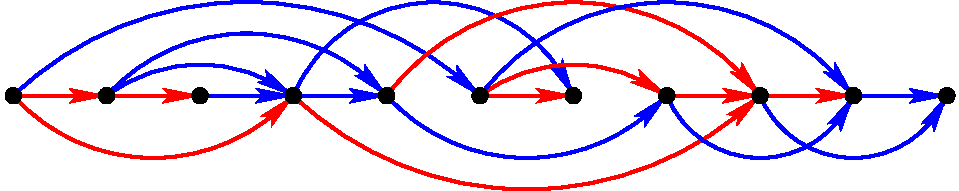
\includegraphics[width=\unitlength,page=1]{respostas/21_grafo.pdf}}%
    \put(0.98846278,0.06679875){\color[rgb]{0,0,0}\makebox(0,0)[lt]{\lineheight{1.25}\smash{\begin{tabular}[t]{l}$z$\end{tabular}}}}%
    \put(-0.0020552,0.06702944){\color[rgb]{0,0,0}\makebox(0,0)[lt]{\lineheight{1.25}\smash{\begin{tabular}[t]{l}$p$\end{tabular}}}}%
    \put(0.09591444,0.06701983){\color[rgb]{0,0,0}\makebox(0,0)[lt]{\lineheight{1.25}\smash{\begin{tabular}[t]{l}$q$\end{tabular}}}}%
    \put(0.19245584,0.06686864){\color[rgb]{0,0,0}\makebox(0,0)[lt]{\lineheight{1.25}\smash{\begin{tabular}[t]{l}$r$\end{tabular}}}}%
    \put(0.29154197,0.05085898){\color[rgb]{0,0,0}\makebox(0,0)[lt]{\lineheight{1.25}\smash{\begin{tabular}[t]{l}$s$\end{tabular}}}}%
    \put(0.38770429,0.06722658){\color[rgb]{0,0,0}\makebox(0,0)[lt]{\lineheight{1.25}\smash{\begin{tabular}[t]{l}$t$\end{tabular}}}}%
    \put(0.48495918,0.06684231){\color[rgb]{0,0,0}\makebox(0,0)[lt]{\lineheight{1.25}\smash{\begin{tabular}[t]{l}$u$\end{tabular}}}}%
    \put(0.58256316,0.06709827){\color[rgb]{0,0,0}\makebox(0,0)[lt]{\lineheight{1.25}\smash{\begin{tabular}[t]{l}$v$\end{tabular}}}}%
    \put(0.68017119,0.05058472){\color[rgb]{0,0,0}\makebox(0,0)[lt]{\lineheight{1.25}\smash{\begin{tabular}[t]{l}$w$\end{tabular}}}}%
    \put(0.77719442,0.05044547){\color[rgb]{0,0,0}\makebox(0,0)[lt]{\lineheight{1.25}\smash{\begin{tabular}[t]{l}$x$\end{tabular}}}}%
    \put(0.89065104,0.06694284){\color[rgb]{0,0,0}\makebox(0,0)[lt]{\lineheight{1.25}\smash{\begin{tabular}[t]{l}$y$\end{tabular}}}}%
  \end{picture}%
\endgroup%

    \caption{}
\end{figure}

\subsection{a} Para cada vértice $i$ do grafo acima, indique os valores $\azul[i]$ e $\verm[i]$ (alguns valores estão preenchidos).

\itemdsep[0.25]

\begin{table}[H]
    \centering
    \begin{tabular}{|c|c|c|c|c|c|c|c|c|c|c|c|}
        \hline
        $i$ & $p$ & $q$ & $r$ & $s$ & $t$ & $u$ & $v$ & $w$ & $x$ & $y$ & $z$ \\
        \hline
        $\azul[i]$ & & & & & & 2 & 0 & 2 & 1 & 1 & 0 \\
        \hline
        $\verm[i]$ & & & & & & 4 & 0 & 2 & 2 & 0 & 0 \\
        \hline
    \end{tabular}
\end{table}


\itemdsep

\subsection{b1} \label{sec:2b}
Descreva uma recorrência que relaciona $\azul[u]$ em função de $\azul[v]$ e $\verm[v]$ para $v \in \Adj[u]$.

\itemdsep[0.25]

Se $cor(u, v) = \text{azul}$, então o caminho $(u, v)$ é válido é começa com aresta azul. Além disso, para qualquer caminho válido $(v, \ldots)$ partindo $v$, podemos juntar $u$ fazendo o caminho $(u, v, \ldots)$, que continua válido e começa com aresta azul. Como $v$ tem $\azul[v] + \verm[v]$ caminhos válidos não-triviais, podemos encontrar $\azul[u]$ por:

\begin{equation*}
    \azul[u] = \sum_{v \in \Adj[u]} \begin{cases}
        1 + \azul[v] + \verm[v] &\text{ se } \cor(u, v) = \text{azul} \\
        0 & \text{ caso contrário }
    \end{cases}
\end{equation*}


\itemdsep

\subsection{b2} Descreva agora uma recorrência que relaciona $\verm[u]$ em função de $\azul[v]$ e $\verm[v]$ para $v \in \Adj[u]$.

\itemdsep[0.25]

\begin{align*}
    \verm[u] &= \sum_{v \in \Adj[u]} \begin{cases}
        1 + \azul[v] &\text{ se } \cor(u, v) = \verm \\
        0 & \text{ caso contrário }
    \end{cases} \\
    &= \abs{(\verm)\Adj[u]} + \sum_{v \in (\azul)\Adj[u]} \azul[v]
\end{align*}


\itemdsep

\subsection{c} Escreva um pseudo-código de um algoritmo de complexidade $O(V +E)$ que recebe um grafo orientado acíclico $G$ representado por listas de adjacências e um vetor \textbf{cor} de cores e devolve um vetor $val[~]$ indexado por $V$ tal que $val[u]$ é o número de caminhos válidos que começam em $u$ para cada $u \in V[G]$.

\itemdsep[0.25]


\newcommand{\Azul}{\const{azul}\xspace}
\newcommand{\Vermelho}{\const{vermelho}\xspace}

\begin{codebox}
\Procname{$\proc{Caminhos-Válidos}(G, \cor)$}
\li \Sejam $\azul[~]$ e $\verm[~]$ vetores indexados pelos vértices em $V[G]$
\li \Para $u \in V[G]$ \Faca        \label{linha:2c:init}
    \Do
\li     $\azul[u] \Recebe \Nulo$    \label{linha:2c:init:end}
        \>\>\>\>\>\Comment usado para marcar vértices não visitados
    \End
\li
\li \Seja $val[~]$ um vetor também indexado por $V[G]$
\li \Para $u \in V[G]$ \Faca        \label{linha:2c:preenche}
    \Do
\li     \Se $\azul[u] = \Nulo$ \Entao
        \Do
\li         $\proc{Caminhos-Azuis-Vermelhos}(\cor, u, \azul, \verm)$    \label{linha:2c:preenche:chamada}
        \End
\li
\li     $val[u] = 1 + \azul[u] + \verm[u]$  \label{linha:2c:preenche:end}
\li     \Comment caminho trivial $(u)$, mais os válidos começando com azul ou vermelho
    \End
\li \Retorna $val$
\end{codebox}

\begin{codebox}
\Procname{$\proc{Caminhos-Azuis-Vermelhos}(\cor, u, \azul, \verm)$}
\li \Comment função que preenche $\azul[u]$ e $\verm[u]$ pelas relações do \textref{sec:2b}{item 2b}
\li
\li $azul \Recebe 0$
\li $verm \Recebe 0$
\li \Para $v \in \Adj[u]$ \Faca \label{linha:2c:calc}
    \Do
\li     \Se $\azul[v] = \Nulo$ \Entao
        \Do
\li         $\proc{Caminhos-Azuis-Vermelhos}(\cor, v, \azul, \verm)$    \label{linha:2c:calc:chamada}
        \End
\li
\li     \Se $\cor[u,v] = \Azul$
        \>\>\>\>\>\>\>\Comment do item 2b
        \Do
\li         \Entao $azul \Recebe azul + 1 + \azul[v] + \verm[v]$
\li         \Senao $verm \Recebe verm + 1 + \azul[v]$ \label{linha:2c:calc:end}
        \End
    \End
\li
\li \Comment salva os valores
\li $\azul[v] \Recebe azul$
\li $\verm[v] \Recebe verm$
\end{codebox}


    \endgroup
    \docline

\end{document}
